\section{Using \priceclass{}es in \Sys}\label{design}

This section describes \sys{} a scheduler that addresses the
\problem{} using \priceclass{}es and meets the \autoref{s:intro}
challenges.

\subsection{\Priceclass{}es}

\Sys{} uses \class{}es to supplant the current interface, which
requires developers to choose an amount of memory per function (which
is then tied to a CPU fraction, \eg{} 0.2 vCPUs).  \Sys{} bills memory
separately and by use, and the price for memory is the same across all
\class{}es.

\Priceclass{}es don't imply absolute guarantees about what resources a
function receives.  The \priceclass{} is instead a metric to express
priority to \sys{}, which \sys{} uses to enforce a favoring of high
\class{} functions.  To avoid the developer-side uncertainty of
bidding wars, \sys{} exposes a fixed set of \priceclass{}es (similar
to how AWS has different EC2 instance types).

\Priceclass{}es are
a metric that has a number of benefits over resource usage
estimations. One is that developers are more likely to have a good
sense of what \priceclass{} a function should have ahead of time,
because they know in what context the function will be
used. \Priceclass{}es also remain the same across different
invocations, whereas resource needs can be heavily skewed in web
applications~\cite{hermod,serverless-in-the-wild}. And finally,
\class{}es more directly align the interests of the developer with
those of the provider, by communicating on the level of what the
provider and developer actually care about: money, and latency (as
achieved by \class{}es in the system).

\Priceclass{}es also allows the provider to provision their datacenters
hardware: by looking at the historical overall amount of high \priceclass{}
load, they know a minimum of how much hardware they need to buy to be able to
comfortably fit that load.

\subsection{Interface}

Developers using \sys{} write function handlers and define triggers
just like they would for existing serverless offerings.  Triggers
assign a \priceclass{} to a function invocation based on the URL
and its arguments. For instance, a simple web application might
consist of a home page view that is assigned a higher \priceclass{}
and costs 2$\mu\cent$ per cpu second, a user profile page view which
is assigned a middle-high \class{} and cost 1.5$\mu\cent$ per cpu
second, and finally an image processing function that can be set to a
low \class{} which costs only 0.5$\mu\cent$ per cpu second.

\Class{}es are inherited across call chains: if a high \class{} function calls a
low \class{} function, that invocation with run with high \class{}. This
inheritance is important in order to avoid priority inversion.

To avoid unexpected costs in the case of for example a DOS attack or a bug,
developers also express a monthly budget that they are willing to pay.~\Sys{}
uses this budget as a guideline and throttles invocations or decreases quality
of service in the case that usage is not within reason given the expected
budget, though it does not guarantee that the budget will not be exceeded by
small amounts.

\subsection{\Sys{} Design}

\begin{figure}[t]
    \centering
      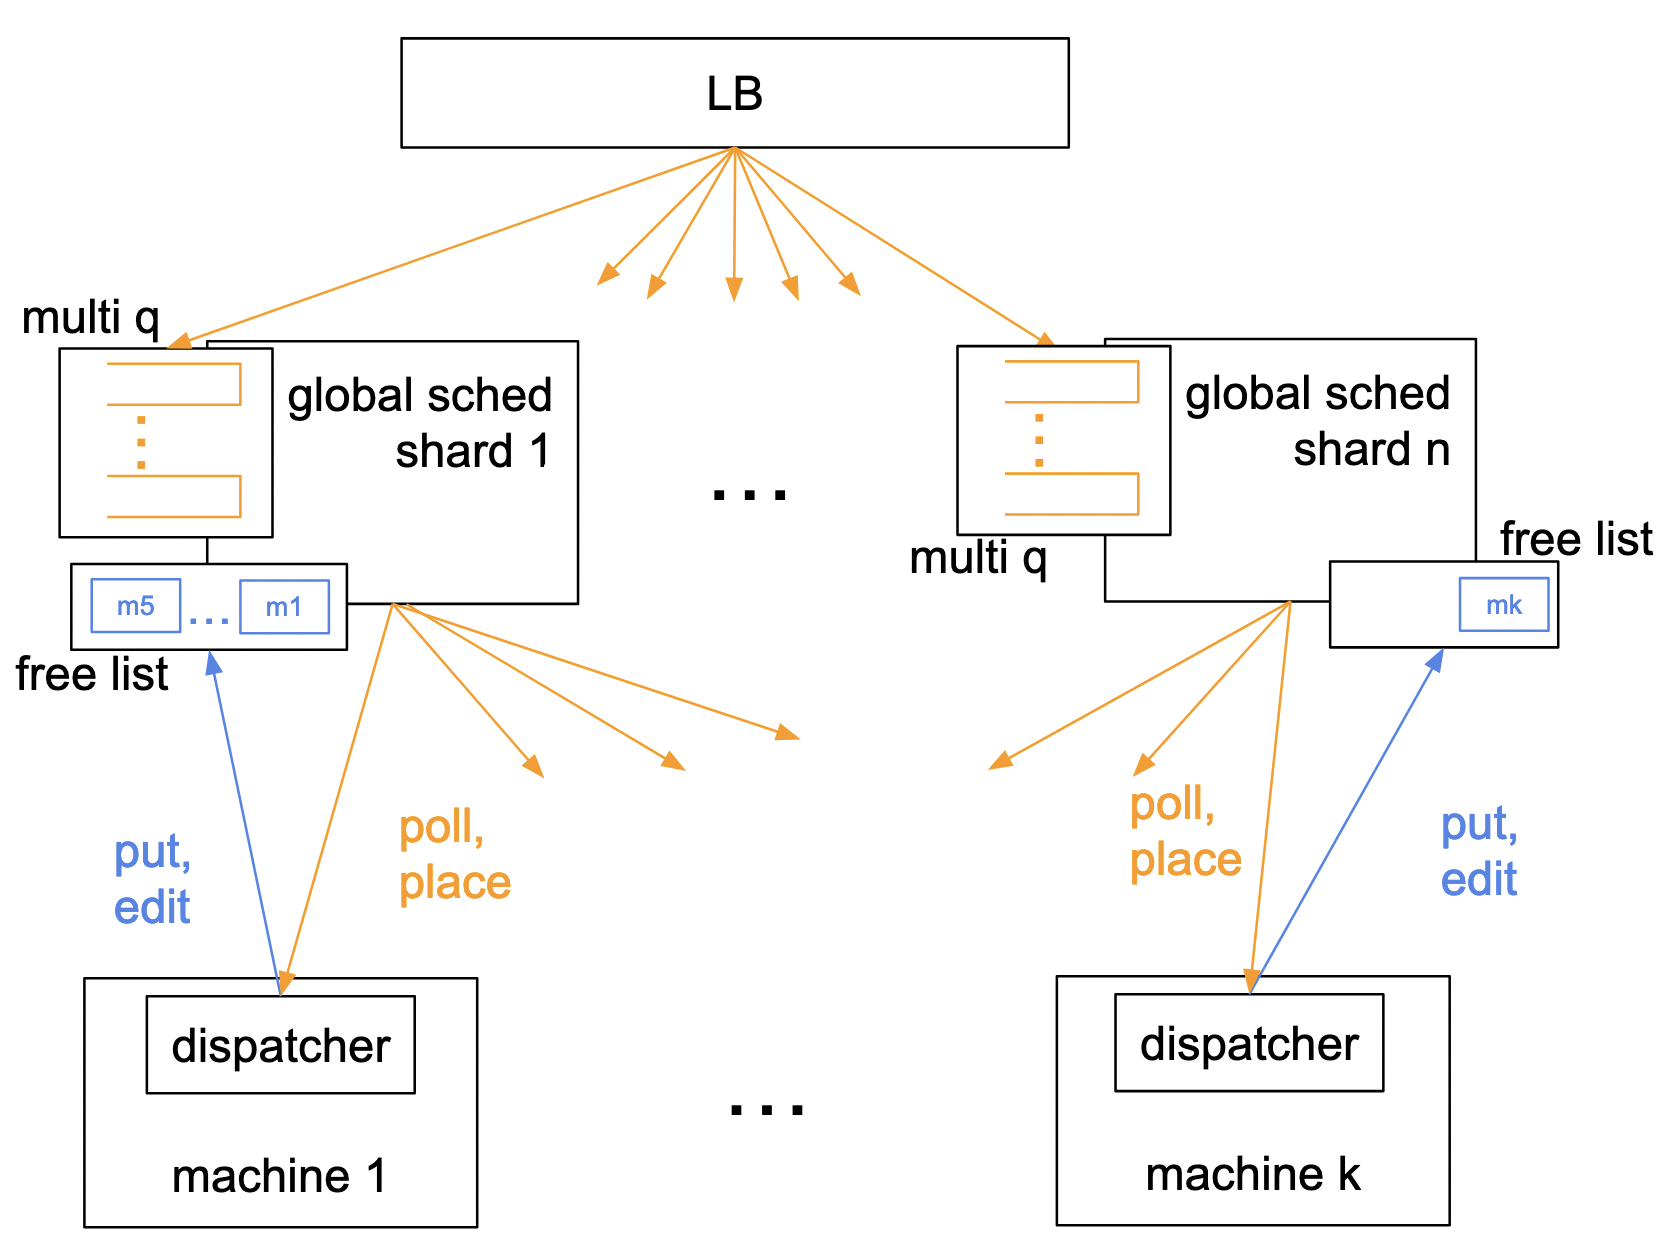
\includegraphics[width=8.5cm]{img/overview.png}
      \caption{ global scheduler shards queue and place functions (in orange),
      on each machine a dispatcher thread keeps track of memory utilization and
      writes itself to idle lists (in blue) }
    \label{fig:overview}
\end{figure}



\Sys{} has as its goal to enforce the \class{}es attached to
functions, which means it needs to prefer higher \class{} functions
over lower ones, and preempt the latter when necessary. As shown in
Figure~\ref{fig:overview}, \sys{} sits behind a load balancer, and
consists of: a \textit{distributed global scheduler}, which places new
function invocations and has attached an \textit{idle list}, a
\textit{dispatcher}, which runs on each machine and communicates with
the global scheduler shards, and a \textit{machine scheduler}, which
enforces \class{}es on the machines.


\textbf{Machine Scheduler.}
The machine scheduler is a preemptive priority scheduler: it preempts lower
\class{} functions to run higher \class{} ones. Being unfair and starving low
\class{} functions is desirable in \sys{}, since image processing functions
should not interrupt a page view request processing, but vice versa is expected.
Within \class{}es the machine scheduler is first come first served. This design
matches Linux' `SCHED FIFO' scheduling~\cite{linux-sched}.


\textbf{Idle list.}  Each global scheduler shard has an idle list,
which holds machines that have a significant amount of memory
available. In the shards idle list, each machine's entry is associated
with the amount of memory available as well as the current amount of
functions on the machine. The idle list exists because datacenters are
large: polling a small number of machines cannot find something that
is a rare occurrence~\cite{join-idle-queue}. The idle list allows the
rare idle machine to make itself visible to the global scheduler. The
idle list also allows the global scheduler to place high \class{}
functions quickly, without incurring the latency overheads of doing
polling to find available resources. This design is inspired by join
idle queue~\cite{join-idle-queue}, but defines idleness via memory
availability rather than empty queues.


\textbf{Dispatcher.}
The dispatcher is in charge of adding itself to a shard's idle list when memory
utilization is low. The dispatcher chooses which list to add itself to using
power-of-$k$-choices: it looks at $k$ shards' idle lists and chooses the one with
the least other machines in it. If the machine is already on shard $i$'s idle
list, but the amount of available memory has changed significantly (either by
functions finishing and memory being freed or by memory utilization increasing
because of new functions or memory antagonists), the dispatcher will update
shard $i$'s idle list.

The dispatcher is also in charge of managing the machine's memory. When memory
pressure occurs, the dispatcher uses \textit{\class{}-based swapping} to move
low \class{} functions off the machine's memory. Having priority scheduling
creates an opportunity: because the dispatcher knows that the lowest \class{}
functions will not be run until the high \class{} functions have all finished,
it can swap its memory out knowing it will not be needed soon. The dispatcher
swaps the low \class{} function back in when the memory pressure is gone and the
function will be run.

\Sys cannot bound the amount of swap space required since it doesn't
ask functions for a memory bound.  In the rare case that \sys runs it
resorts to killing low-class functions.  Providers can estimate the
amount of swap space required by looking at memory utilization and
since the SSDs necessary for swap space are
inexpensive~\cite{ssd-price} we expect that killing is rare.

\textbf{Global Scheduler Shards.}
Global scheduler shards store the functions waiting to be placed in a multi
queue, with one queue per \priceclass{}. Shards choose what function to place
next by looking at each function at the head of each queue, and comparing the
ratio of \class{} to amount of time spent in the queue. This policy ensures
that high \class{} functions don't have to wait as long as low \class{}
functions to be chosen next, but low \class{} functions will get placed if they
have waited for a while.

When placing the chosen function, the shard will first look in its
idle list. If the list is not empty, it will choose the machine with
the smallest queue length.  If there are no machines in the idle list,
the shard switches to power-of-$k$-choices: it polls $k$ machines, and
chooses the least loaded machine (by number of functions running).
